\documentclass[11pt, a4paper]{article}

\usepackage{cite}

\usepackage{booktabs}
\usepackage{siunitx}
\DeclareSIUnit{\calorie}{cal}

\usepackage{pgfplots}
\usepackage{pgfplotstable}
\pgfplotsset{compat=newest}

\usepackage{physics}

\usepackage{amsmath}
\usepackage{tikz}
\usetikzlibrary{positioning, calc}

\pgfmathsetmacro{\s}{0.5}
\pgfmathsetmacro{\r}{0.5cm}

\usepackage[caption=false]{subfig}


\title{Predicting the binding free energy of DNA intercalators}

% \author{Student 14016005 | CHEMGM01}

\setcounter{tocdepth}{3}

\begin{document}

% \maketitle

% \tableofcontents

\section*{Abstract}

Planar aromatic molecules can interact with DNA chains by intercalating between consecutive basepairs. Once intercalated they can cause mutations during gene expression resulting in cancerous cells. This same mechanism renders some of these molecules good anti-cancer treatment if targeted correctly. The efficacy of intercalators is therefore of importance to the pharmaceutical industry. However due to forcefield inadequacy and the slow convergence of computational simulations, the application of well established binding free energy calculation methods to DNA-intercalator system to predict efficacy has been low in number compared to protein-ligand studies. Here we apply the three main methods to predicting efficacy via computational methods to DNA intercalator systems comparing results to experiment. We found that docking methods are capable to distinguish between intercalators that have different scaffold structures, MMPBSA type simulations can correctly rank a congeneric series of intercalators, and formally exact methods predict the binding affinity of intercalators with root mean squared error of 0.41 kcal/mol. The correct preparation of the models was also important, and to this end we developed computational tools to automate the correct setup stages. With an automated setup and deployment tool and running our protocols we think will start to probe a wide range of intercalators to investigate their interaction and efficacy with DNA.

\section{Introduction}

% \section{DNA and intercalation}

Shortly after the unraveling of the complex structure of the double stranded DNA that self-assembles into a helical form started the exploration of ligands that form complexes the DNA in a diverse set of binding forms. Certain molecules could bind to DNA grooves, or intercalate between DNA basepairs. Of these two main categories of binding, the former is less of interest and hence less studied. Intercalators have a wide range of interest and use cases, including cancer treatment, due to their varied binding properties to DNA. The existence of intercalators was first predicted and later confirmed by Lerman et al. whereby a small planar aromatic molecule inserts between consecutive DNA-base pairs, perturbing the local structure of the DNA, but still having a stabilising effect through base pair stacking. Intercalation can potentially explain, and aid in understanding a number of DNA specific phenomena including transcription, mutation, and the mechanism of certain anti-tumour agents, like the anti-cancer agent small molecule acridine. Intercalator can be neutrally charged or cationic, they disrupt the continuous and predictable flow of the genetic information encoded in the base-pairs. In contrast other forms of DNA binding, major or minor groove, or electrostatic binding, does not deform the structure, and has a smaller effect of the function of DNA. Intercalation greatly changes the structure of DNA, including the base pair distance, decreasing the twist angle by up to 50\%, essentially unwinding the DNA to some extent in the local neighbourhood of the intercalation site. In order to accommodate the molecule, the inter-basepair distance has to be increased, sometimes up to double its original size. The increase in separation elongates the whole DNA helix. Moreover while the DNA helix unwinding compensates for the insertion maximising the base stacking and hence the stability, the backbone structure, for example the distance between consecutive phosphate groups remains nearly identical. This level of perturbation and the fact that it is reversible (as the binding is non-covalent) provides a basis for a wide range of applications.

% Application and importance in drug treatment of intercalators

The importance of intercalators in drug design and the potential application of these to treat a wide range of cancer has already been shown by certain compounds and FDA approved treatments. Two similar compounds, doxorubicin and daunomycin, are currently used as anti cancer treatment for more forms of cancer than any other compound. Intercalation of these compounds disrupts replication and transcription of DNA and leads to the death of cancerous cells. Once the crystal structure of this complex was determined with X-ray diffraction methods, the mode of action was revealed to be that of intercalation, as the fused ring system is indeed sandwiched between basepairs. The mechanism was theorised to be a ring-insertion with the inter-basepair distance increasing, but certain structural features staying the same for example the hydrogen bonding.

% Talk something about the kinetics including the metadyanmics based approaches. This is starting to place out study in the context of the larger fiels. Thank you! 

The basepair distance opening and molecule insertion nonetheless is too simple of mechanism, and certain high quality experimental measurements indicate a more sophisticated binding mechanism. For example, kinetic measurements indicate a three step intercalation process, with the first step being a fast binding to the outside of the DNA chain, and the second and third slower conformational adjustments. However the experiments are low resolution and the hypothesis of the intercalations is not fully elucidated. Certain computational techniques have been used to investigate this mechanism. Metadynamics and umbrella sampling can provide atomic-scale resolutions and free energy estimates of the intercalation mechanism. They confirm the earlier studies, that the process is composed of three steps, an initial binding in the minor groove of the DNA, followed by the rotation of the drug and DNA deformation into a seconds intermediate metastable state, and finally separated by only a small barrier complete rotation of the molecule into the space between basepairs to establish a full basepair stacking interaction.

% 





% \section{DNA modelling and molecular dynamics}
% 
% \subsection{Atomistic modelling}
% 
% The structure of biomolecule, like DNA is complex and interesting. How can we gain insight into the  composition of structures like this on an atomic level? Experimental techniques, like CryoEM \cite{bai2012cryo}, x-ray crystallography or NMR provide information about the composition at a resolution small enough to distinguish atoms, and some methods also provide dynamical properties too. However, certain phenomena or physical property is simply out of the reach of these experimental techniques. In silico techniques, such as molecular dynamics \cite{cheatham1995molecular}, can provide insight otherwise not accessible to experimentalists. The focus of this thesis is applying such in silico methods to bio-molecular systems, with a particular emphasis on molecular dynamics. 
% 
% Nonetheless, as a starting model, even in silico methods take data from experiment, therefore it is briefly described here.
% 
% \subsection{Experimental models}

The structure of DNA and other biological molecules can be determined in a number of ways including X-ray, NMR and Cryo-EM. Unfortunately, it is not always possible to determine the structure of the desired system under investigation experimentally. In that case it might be the case that we can use our knowledge of similar structure and modelling to generate new structures that are likely to resemble reality. Here we briefly describe these techniques.

\subsubsection{X-ray crystallography}

The most notable method, especially from a historical point of view, to analyse the structure of DNA is by X-ray diffraction. This method lead to the discovery of the basic double helical structure of the DNA strand. The resolution is determined by the wavelength of the radiation used to investigate the structure. In case of biologically relevant molecules we want to distinguish between atoms, therefore a sub 1 angstrom resolution is required. This resolution corresponds to a wavelength of X-ray radiation. To produce a high quality image a regular array of units to scatter the radiation is required. This means that we have to crystallise the molecule, which places it into a state somewhat different from the biological conditions it was in originally.


% 
% \subsection{Computational modelling}
% 
% Simulating a system via computational methods requires an initial model, where by model, we refer to the coordinates of every particle in the structure of interest. If, for example, we want to simulation nucleic acid structures, then the model is the three dimensional coordinate of every atom in the DNA structure. In general the model can be build in one of two ways: by hand de novo, or using another source (experimentally derived structures for example). The quality of the initial starting structure can have a large effect on the computational results and the validity of the simulation. This will become apparent in the results section, where two similar systems were simulated with different levels of initial structure validity.   
% 
% \subsubsection{Quantum mechanics}
% 
% In a quantum mechanical (QM) description of a system, the electrons are explicitly accounted for as they are the fundamental particles of this level of description. The energy of the system is calculated as the interaction energy between electrons based on electronic structure calculations. There are few (if any) empirical or fitted parameters in these models, but the underlying physical description is sometimes approximated for tractability. Usually QM calculations are very expensive and scale cubic (or worse) with the number of electrons in the system \cite{vsponer1996hydrogen}.
% 
% \subsubsection{Molecular mechanics}
% \label{sec:mm}
% 
% In molecular mechanics (MM) the description is based on particles corresponding to atoms. Every atom in the system has a number of parameters defining the interaction between other particles, including a partial charge, bond, angle and torsion parameters, and non-bonded interaction parameters. These parameters are all empirically determined (fitted to experimental observables, quantum mechanical calculations, or other data). MM simulations are faster than quantum calculations, hence why this study was conducted using MM methods to simulate our DNA based systems. Some of the limitations of MM methods, including lower accuracy and the lack of the ability of bond rearrangement was considered, and determined to be a non issue for the systems at hand. Furthermore, QM simulations are too expensive to run for adequate amount of time (nanoseconds of simulations) that is required to reach and sample the equilibrium state. The size of the system is also an important decision factor in choosing between QM and MM. Roughly speaking, QM simulations have on the order of a couple of hundreds of atoms, while MM simulations are routinely run with tens of thousands of atoms \cite{leach2001molecular, frenkel2001understanding}.
% 
% \section{Theoretical details of molecular simulations}
% 
% Simulating molecular systems is, at a high level, very simple and straight forward. First, build a particle based description of the system, where particles are the only entities that can interact with each other or the environment. Then, based on rules, propagate the system through time starting from some initial state (as described before the state of a system is the position and velocities of every particle) for a given number of steps or iterations. The rules by which you propagate the system can be either deterministic or random. As you build up a collection of consecutive states of the simulated system, certain properties can be calculated per frame (frame being a state in the context of a simulation) or averaged over multiple states to get ensemble estimates over time. 
% 
% There are two main categories of molecule simulations based on the nature of the propagation rules: Molecular Dynamics (MD) or Monte Carlo (MC). Molecular dynamics refers to the numerical integration of the equations of motion. They are used to investigate thermodynamic properties as well as structural and dynamical phenomena of the system. Monte Carlo type simulations on the other hand, generate new states based on the current state via probabilistic rules. The set of states generated this way can be used to predict thermodynamic and structural properties, but \emph{not} dynamical ones. This is because a MC simulation has no concept of time by which states are ordered and evolved.
% 
% % \subsection{Equation of motion}
% 
% \subsection{Forcefield}
% 
% The molecular mechanics model described in section~\ref{sec:mm} is based on a number of interatomic potential energy functions. All these potential energy functions have a number of constants, the values of which are fitted to higher level calculations or experiment.
% 
% In order to have credibility in the theoretical models that are used to predict experimental measurements, or more drastically, substituting them, we have to validate the force fields that are used in the molecular dynamics simulations. In particular, the last generation of force-fields for DNA systems specifically has raised questions about their validity especially at longer simulation timescales. It was found that while not all theoretical simulations are equally reliable, the latest generation of force fields of the AMBER family designed to model DNA (BSC1 \cite{ivani2016parmbsc1} and OL15 \cite{zgarbova2015refinement}) can be safely used to reproduce the global structure of DNA, and predict observable quantities of interest, like the free energy of binding. They provide the most accurate results when comparing MD trajectory simulation data to experimental observables like NMR structure of X-Ray resolved structures. Furthermore, these forcefields reproduce experiments in an unbiased environment, and a common technique to force DNA trajectory to align with experimental data, termed restrained MD, is not essential for this study.
% 
% \subsection{Main steps in a molecule dynamics simulation protocol}

Every system that is investigated via simulation method required specific care, but there are four steps that are present in most molecular dynamcs workflows. They are not hard written rules, but following these steps assures that the system is correctly equilibrated and sampled during simulations, and also minimizes the chance that the energy of the system gets out of control.

The four steps are: system preparation, minimisation, equilibration and production.

\subsubsection{Minimisation}

During minimization or relaxation, we want to find a local minimum of the biological system so that during the start of the molecule dynamics simulation the system does not end up in an unstable state (sometimes termed ``blow up'') This can happen due to forces on certain atoms being too large at the start, and they were to move too much during the first couple of timesteps of the simulation. To achieve this standard minimisation algorithms are employed, sich as steepest descent or the fire minimiser. 

\subsubsection{Assignment of velocities}

As discuss before, minimisation takes the system to a state where we can start the numerical integration of the equation of motion without the possibility that any subsequent displacement will be too large or physically unrealistic,  however, minimisation only takes into account the positions of every particle, and does not change the velocities, therefore we have to set the velocity vectors of every particle separately at the start of the simulation. Thus, to set the starting velocities one usually assigns random initial velocities to atoms in a way such that the correct Maxwell-Boltzmann distribution at the desired temperature is achieved as a starting point. The actual assignment process is typically unimportant, as the Maxwell-Boltzmann distribution will quickly arise naturally from the equations of motion. The last particle in the simulation box is typically given a velocity such that the centre of mass momentum is zero, and the simulation box itself as a whole does not drift with time. This is because in Newtonian dynamics the momentum of the centre of mass is conserved. 

Single simulation trajectories are somewhat meaningless, and in most cases, we want to run a set of independent simulations, of different replicase or realisations of the a particular system. This is to assess the error on the particular observable, and collect statistical descriptors like the spread, mean and standard deviation, or help understand how the starting structure effect the results. 
It is important to note, that even the smallest difference in the inital conditions of the system (for example the position of a single atom, or magnitude of velocity) can lead to completely divergent results after some simulation time, meaning that simply running different simulations starting with different initial velocities will lead to completely different time evolution over a long enough simulation. An even better approach to generating different initial replicas, is to start from completely different conformations such as different conformations of the molecules simulations, different binding pose in a receptor ligand simulation, as this will lead to divergence right from the beginning of the simulation.

\subsubsection{Equilibration}

In order to compare the data generated by simulation to experiment, we usually want to bring the simulation conditions to experimentally comparable values (including, temperature, pressure, energy) which requires simulations in a specific ensemble (NVE, NPT, etc.). Data collected should not be biased by the initial conditions on the simulation either. Therefore we need to run the simulations for some period of time until the the system is at the appropriate state, as well as relaxed from any metastable state introduced by the starting state of the simulation. In other words we are interested in sampling the most likely, equilibrium state of the system in the given ensemble. In case of biomolecules it is important to bring them to a configuration that is relevant and could take a long simulation time to reach such state.

The first step in the equilibration phase is to bring the system to the desired thermodynamic state. By thermodynamic state we mean a given temperature are pressure. Assigning velocities with the correct distribution does set the inital temperature, but the thermostat will still have to partition the kinetic and potential energy of the system correctly. To this end, a thermostated equilibration period is run before collecting data even in the case of the NVE ensemble. To monitor the equilibration phase, we look at the temperature, pressure, kinetic and potential energy of the system over time and monitor their fluctuations. A simulation is siad to have equilibrated when these parameters reach a stead state and only fluctuate around that value with minial drift. This definition while not perfect, is a good measure of equilibration of a system to a given pressure, temperature, simulation box (i.e. volume) or energy.

Other properties of the system of interest should not change too during simulation. This is harder to monitor then the thermodynamic properties discussed above. Even at equilibrium the system might undergo slow fluctuations especially if it has slow degrees of freedom, but the values should stay around a specific value. The bio-molecular system it is common to investigate the root mean squared deviation of the particles over time. and potentially other properties like the number of hydrogen bonds between the biomolecules present and water, as these may be slower to equilibrate than system-wide properties like the temperature and pressure.

Once the energy component and other properties fluctuate around constant values with minimal or no drift we have reach the end of equilibration. If some of the properties of interest exhibit a systematic drift with time, that the system has probably not equilibrated sufficiently. 

The target ensemble introduces a difference in the equilibration protocol.  In the NVE ensemble the thermostat should be removed and frame of the system should be selected that is as close to the desired kinetic and potential energy as possible. The frame containing the positions and velocities of every particle is used to start the production simulation at the correct temperature. This is because the temperature fluctuates over the simulation when coupled to a thermostat.

If the target is the NPT ensemble (that is the most common for biological simulation) then the system should first be relax to the desired temperature in the the NVT ensemble, then the barostat turned on to relax the simulation box to the desired pressure.

\subsubsection{Production}

Once the system has equilibrated we can step into the final stage where we collect the data about the system. This phase of the workflow is called production. The main difference between the end of the equilibration and the production run is that in production we keep and analyse the data produce as opposed to discarding it. Production always comes after a rigorous equilibration phase in the correct ensemble, and it should never be collected after a sudden change of any of the properties of the simulation, like the simulation box size, temperature, pressure (unless this is the goal of the simulation).

If the ensemble changes from equilibration to production, then it is advised to discard the initial data collected even in the production simulation (for example switching from NPT to NVT) with the usual considerations about equilibrium still applicable here.

Analysis of the production work required special care as some of the observable are not trivial to calculate, and the error on these values must be correctly estimated. Usually, analysis involves calculating the expectation values of certain observables, with the important consideration that these values are converged, meaning that they no longer depend on the further length of the simulation (or replica of simulations) or on the initial conditions that the simulation was started from. This is very much related to the equilibration discussed above, with the difference being what is the subject at hand. Depending on the time to relaxation, it is common to realise that the system was not equilibrated after analysis of the production run.

A key consideration is the storage and frequency of storage of the simulated data. Storing data very frequently (for example storing at every timestep) can be tempting, but limits in the physical availability of storage space is usually a limiting factor, but also the additional information contained in snapshots close together diminished drastically as the time separation become small. In particular in molecular dynamics simulations consecutive frames are correlated, so storing and analysing each frame is essentially redundant and adds no value or insight to the calculation of a specific observable. Therefore, storing data more frequently than the autocorrelation time is not necessary. Disk space should also be taken into consideration. Depending on the size of the system (the number of particles) the size of a single frame in a trajectory can be large. But even if disk space is not an issue, storing snapshots with an autocorrelation frequency should be enough.

There are various strategies to reduce size of the data. One can store reduced precision of the coordinates, or chose to save with different frequency the component of interest. For example because energy is much smaller to store, it can be storied with a higher frequency then trajectory coordinates. This depends on the analysis at hand.


% 
% \subsection{Thermostat}

Thermostats are ofter used in molecular dynamics simulation to control the temperature. MD simulations are used to understand, observe and predict the properties of interest for a given system. If we want to compare to results done in laboratory conditions (where temperature is usually constant) we have to sample the canonical ensemble. Therefore the temperature of the system must be maintained at a certain level, and a thermostat should be used.

To determine the temperature of a molecular dynamics simulation we can use the equipartition theorem involving the kinetic energy of the system

\begin{equation}
  \frac{3}{2} N k_b T = \langle \sum_{i=1}^{N} \frac{1}{2} m_i v_{i}^2 \rangle
\end{equation}

The temperature is a time averaged quantity indicated by the brackets, meaning that it is an average over many snapshots of the simulation. Applying the equipartition theorem to just a single snapshot of the simulation, we get the instantaneous temperature. The instantaneous temperature is usually not equal to the desired ensemble temperature, but it should fluctuate around that value, the target temperature.

In general, thermostat work by altering the Newtonian equations of motion, which inherently conserve the energy. Therefore one should not use a thermostat if the desired property is dynamical (for example the diffusion coefficient); but instead, the thermostat is used to bring the system to the desired temperature then turned off. While thermostats give non-physical dynamics, some have less effect on particular dynamical properties and are save to use in molecular dynamics simulations.

There are two ways to categories thermostats: (i) they can be either deterministic or stochastic depending on whether they use random numbers to alter the equations of motion or (ii) global or local based on the extent of the effect, whether its on the full system or just a subset of the particles. Thermostats also differ in the algorithm used to control the temperature. Certain thermostats operate by rescaling the velocities of the particles outside the dynamics, by applying the change after a simulation timestep has happened and the coordinates and velocities have been updated. Others include implicit or explicit collisions with an external heat bath.

\subsection{Barostat}

Thermodynamic properties of interest are measure inside laboratory condition, therefore, at short timescale the system is under constant temperature \emph{and} pressure. The pressure is usually at atmospheric pressure, unless some form of pressure control is used, for example a piston, inert gas, etc. This set of conditions is part of the isothermal-isobaric ensemble, probably the most common ensemble in molecular dynamics simulation, especially that of biologically relevant systems. Similar to thermostat, if the pressure in the system needs to be constant, a barostat algorithm should be used.

Barostats control the pressure if the system, so if the aforementioned isothermal-isobaric ensemble is desires, that they must be used in conjunction with a thermostat. Without one, we would be in a isoenthalpic-isobaric ensemble, where only the number of particles, the pressure and the enthalpy  of the system is constant.

The background if barostat is analogous to that of thermostats. The virial theorem is used to measure the pressure in a molecular dynamics simulation. In the case of periodic boundary conditions and pairwise interactions, other equations are considered. Nonetheless, these formulas also provide pressure as a time averaged quantity over the simulation range. The pressure calculated just from a single snapshot is termed the instantaneous pressure. Similarly to temperature, the instantaneous pressure is not equal to the target, but fluctuates constantly around that value during the simulation.

To model the idea of a barostat, consider a system that is compressed/expanded by a hypothetical piston from every direction with a uniform force. Since it is acting from all directions it can be considered that the compression is uniform. The mass of the piston can be changes to correspond to stronger compression force. This changes the frequency with which particles interact with the system enclosure. These impacts on the simulation box can be related to the stress the surrounding is applying to the system.

\subsection{Integrators}

Any system with more than three interacting bodies has a solution to their equation motion that cannot be analytically derived. Instead, approximation have to be introduced to the dynamics of a system by numerical methods in a discrete manner, termed numerical integration of the equations of motion. The algorithms that perform such numerical integration are called integrators. A key criteria for any integrator is energy conservation at short and long timescales.

There are certain feature that integrators should have in order to be effectively used in molecular dynamics simulations. To start with, the integrator should introduce little error in the dynamics of the system. By definition integrators use discretisation to approximate the dynamics of the continuous motion, therefore they will introduce an error because of this approximation. Alongside discretisation errors, an additional source of error comes from truncating the numbers as they are stored in computers to a fixed precision. There are many strategies to reduce discretisation error, while truncation error can be reduced by increasing the precision of the floating point numbers used by the computer code.

By minimising the discretisation error, we want to minimise errors in the phase space volume and conserve the energy during simulation. If phase space volume changes over the simulation, then the system is, by definition, is a different ensemble from one timestep to the next. This means that the data collected during simulation is from different ensembles. One simple solution is to guarantee that the integrator is reversible. If the operator that propagates the system preserves phase space, then by definition is also reversible, in other words the operator is applied to a state stepping $\delta t$ forward, and then applying the same operator $-\delta t$ step, and the system remains the same, than we have reversibility and hence phase space volume conservation. 

% \section{Free energy calculations}
% 
% \subsection{Binding constant and equilibrium}
% 
% Planar aromatic molecules containing a fused ring system scaffold can intercalate between consecutive DNA base pairs. They are termed intercalators. Whilst there are cases when intercalators form covalent bonds with the DNA base pairs this is an irreversible process. If the bonding is facilitated via non-bonded interactions only ($\pi$ stacking), then the interaction is reversible \cite{berg2002biochemistry}. The study here is only concerned with the later intercalation type, as this is the more common form and the tools used (molecular mechanics) are suited to model this type of interaction only. In a solution containing double stranded DNA fragments and the intercalator, they will be constantly interacting, with the intercalator binding and unbinding from the DNA. This process can be modelled by a reversible chemical reaction
% 
% \begin{equation}
%   A + B \underset{k_1}{\stackrel{k_{-1}}{\rightleftharpoons}} AB
% \end{equation}
% 
% where the rate constant of the forward and backward reaction are the intercalation and de-intercalation reaction rates respectively. In equilibrium the two rate equal, therefore the concentration of each component (DNA, intercalator, and complex) is constant. The association constant $K_a$ is determined by the concentrations at equilibrium, and is given by
% \begin{equation}
%   K_a = \frac{k_1}{k_{-1}} = \frac{[AB]_{eq}}{[A]_{eq} [B]_{eq}}
% \end{equation}
% 
% \subsection{Thermodynamics: the binding affinity}
% 
% One can interpret the process of intercalation as the reaction to minimise the appropriate thermodynamic potential for the given ensemble \cite{adkins1983equilibrium}. The most common ensemble for the experimental conditions is the NPT ensemble, because the number of molecules, pressure and temperature are constant. The associated potential if the Gibbs free energy, $G$, given by
% 
% \begin{equation}
%   G = U + pV - TS = H - TS
% \end{equation}
% 
% The intercalation will happen spontaneously if the difference in free energy ($\Delta G$) between the intercalator and DNA in free state and the complex is negative. The intercalation then will happen until the free energy is minimised and equilibrium has been reached. This difference can be calculated as
% 
% \begin{equation}
%   \Delta G = G(complex) - G(DNA) - G(intercalator)
% \end{equation} 
% 
% The numerical value corresponding to the strength of binding, with more negative values being stronger binders. The change in free energy can also be related to the aforementioned equilibrium constant $K_a$ via the van't Hoff equation
% 
% \begin{equation}
%   \Delta G = - R T \log K_a
% \end{equation}
% 
% This means that the temperature and the free energy difference are closely related. If the temperature increases then the concentration of the complex also increases at the equilibrium. The value of $\Delta G$ is often called binding affinity or free energy of binding. The two terms can be used interchangeably. For certain use cases it is meaningful to break down the free energy difference into an enthalpic and entropic component
% 
% \begin{equation}
%   \Delta G = \Delta H - T \Delta S
% \end{equation} 
% 
% \section{Computational methods for free energy calculations}
% 
% An approach to calculating the binding free energy is via computational techniques. This method form the basis of this thesis. To compute the free energy this way offers a number of advantages over investigating the system experimentally. Molecules that cannot be synthesis can be simulated in silico, and we can study systems at an atomistic level. Molecular simulations provide this level of detail, but in order to calculate the macroscopic properties (like the free energy \cite{macke1961ld}) we have to use statistical methods to derive them from the the microscopic simulations.
% 
% \subsection{Theoretically exact free energy methods}
% 
% There are a number of formally exact methods to calculate the free energy from simulation. By exact we mean that it contains to empirically fitted parameters in the equations. Two of the main techniques are called free energy perturbation (FEP) which is based on exponential averages of the change in the potential energy, and thermodynamic integration (TI) which is based on integrating the system as it changes from one state to another through an alchemical pathway \cite{chipot2007free, deng2009computations}. Due to considerations in computational efficiency, the theoretically exact calculations compute free energy \emph{differences} simulated via non-physical system transformations (known as alchemical transformations). A thermodynamic cycle can illustrate how these alchemical changes can be related to relative differences which are of real interest
% 
% \subsubsection{The thermodynamic cycle}
% 
% Free energy is a function of state and as such cumulative variations around a closed thermodynamic cycle sum to zero. Figure~\ref{fig:tiescycle} depicts such a cycle which could be used to calculate the relative binding affinity, $\Delta \Delta G$, of two different intercalators to the same target where
% 
% \begin{equation}
%   \Delta \Delta G_{intercalation} = \Delta G_{a} - \Delta G_{b} 
% \end{equation}
% 
% The vertical arrows show the intercalation of two molecules A and B, to the DNA, with free energy differences $\Delta G_{a}$ and $\Delta G_{b}$. This path involves substantial rearrangement of the DNA chain to accommodate the molecules, and the simulation would take a long time to converge. The horizontal paths describe the free energy differences associated with the change of molecule A into molecule B in the intercalated and free state respectively. While converting one molecule into another is not physical, it can be achieved in a computer simulation. If the two molecules are similar in composition, then the relative rearrangement in the DNA with will small, and the simulation will converge quickly. We can use the fact that the free energy is a state function to calculate the relative free energy of binding as
% 
% \begin{equation}
%   \Delta \Delta G_{intercalation} = \Delta G_{1} - \Delta G_{2} 
% \end{equation}
% 
% It path taken does not matter as the difference in the free energy of the intercalated state of the two molecules is independent of it. The path taken is represented by introducing an alchemical variable into the Hamiltonian called $\lambda$ that takes on values between $[0, 1]$. Then, the only constraint on the hamiltonian is that at $\lambda = 0$ is corresponds to the molecule A only, and at $\lambda = 1$ to molecule B. A similar approach can be applied in the investigation of mutating the DNA sequence but keeping the intercalated molecule the same.
% 
% State be need not be a molecule, but the absence of one too. In this case the free energy of the absolute binding is calculate in much of the similar manner as the relative free energy is calculated with minor differences.
% 
% \begin{figure}
%   \centering
%   % \documentclass[margin=0.1in]{standalone}
% 
% \usepackage{amsmath}
% \usepackage{tikz}
% \usetikzlibrary{positioning, calc}
% 
% \pgfmathsetmacro{\s}{0.5}
% \pgfmathsetmacro{\r}{0.5cm}
% 
% \begin{document}

\begin{tikzpicture}
  [ 
  waterbox/.style={rectangle,draw=blue!50,fill=blue!10,thick, inner sep=0pt,minimum size=5*\r},
  dna/.style={ultra thick, line cap=round},
  intercalator/.style={dna, dna, line width=3pt},
  pre/.style={<-,shorten <=1pt,shorten >=1pt,semithick}, 
  post/.style={->,shorten <=1pt,shorten >=1pt,semithick}
  ]
  
  \node[waterbox] (a)               {};
  \node[waterbox] (b)  [right=of a] {}
    edge [pre] node[auto, swap] {$\Delta G_1$} (a);
  \node[waterbox] (a') [below=of a] {}
    edge [post] node[auto] {$\Delta G_a$} (a);
  \node[waterbox] (b') [below=of b] {}
    edge [pre] node[auto] {$\Delta G_2$} (a')
    edge [post] node[auto, swap] {$\Delta G_b$} (b);
  
  \node (l1) [below=of a'] {$\lambda=0$};
  \node (l2) [below=of b'] {$\lambda=1$}
    edge [pre] (l1);
    
  \draw[dna] foreach \x in {a.center, b.center, a'.center, b'.center} {
    (\x) [rounded corners=\r] -- ++(-\s, 0) -- ++(0, 2*\s) 
    (\x) [rounded corners=\r] -- ++( \s, 0) -- ++(0, 2*\s)
    (\x) [rounded corners=\r] -- ++(-\s, 0) -- ++(0,-2*\s)
    (\x) [rounded corners=\r] -- ++( \s, 0) -- ++(0,-2*\s)
    
    (\x) ++(-0.866*\s, 0.5*\s) -- ++(1.73205*\s, 0)
    (\x) ++(    -1*\s,   1*\s) -- ++(      2*\s, 0)
    (\x) ++    (-1*\s, 1.5*\s) -- ++(      2*\s, 0)
    
    (\x) ++(-0.866*\s, -0.5*\s) -- ++(1.73205*\s, 0)
    (\x) ++(    -1*\s,   -1*\s) -- ++(      2*\s, 0)
    (\x) ++(    -1*\s, -1.5*\s) -- ++(      2*\s, 0)
  };
  
  \draw[intercalator, blue] (a.center)  ++(-0.8*\s, 1.25*\s) -- ++(1.6*\s, 0);
  \draw[intercalator, red]  (b.center)  ++(-0.8*\s, 1.25*\s) -- ++(1.6*\s, 0);
  \draw[intercalator, blue] (a'.center) ++(-0.8*\s,  2.2*\s) -- ++(1.6*\s, 0);
  \draw[intercalator, red]  (b'.center) ++(-0.8*\s,  2.2*\s) -- ++(1.6*\s, 0);

\end{tikzpicture}

% \end{document}
%   \caption{The thermodynamic cycle illustrating how to calculate the relative binding free energy of two intercalators. The two intercalators (red and blue) bind to the same DNA sequence. The horizontal arrows are the alchemical changes from one intercalator to another, while the vertical arrows represent the independent free energies of intercalator binding.}
%   \label{fig:tiescycle}
% \end{figure}
% 
% \subsubsection{Thermodynamic integration}
% 
% During thermodynamic integration we run a number of independent simulations for different values of $\lambda$. The parameter takes values between 0 and 1, and represent the gradual morphing from molecule A into molecule B. The ensemble average of the derivative of the potential energy with respect to the parameters is numerically integrated to get the free energy difference. 
% 
% \begin{equation}
%   \Delta G = \int_{1}^{0} \langle \frac{\partial V (x, \lambda)}{\partial \lambda} \rangle \partial \lambda
% \end{equation}
% 
% A key difference to FEP is that in TI each average is independent of each other. This means that sufficient simulations need to run to correctly integrate numerically, which increases the computational requirements \cite{chipot2002free}.
% 
% It is important to note, that in TI, the alchemical transformation has to run for both the bound states and the unbound states. Furthermore, the difference in consecutive $\lambda$ windows need to be small. This is necessary in order to provide enough points for accurate numerical integration. In general this requires parallel simulations on the order of ten, each running for as long as convergence is reached. This method is computationally expensive compared to other less accurate methods, more approximate methods.
% 
% \subsection{MMPBSA}

Molecular Mechanics Poisson-Boltzmann Surface Area (MMPBSA) is one of the theoretically approximate methods to calculate the free energy of system \cite{gilson2007calculation, steinbrecher2010towards}. It is the most accurate of the approximate methods, and it has previously been applied successfully to the free energy calculation of various biological systems including protein-ligand and DNA intercalator complexes.

This method is a good choice for comparing and ranking a set of molecule by their binding affinities for two main reasons: MMPBSA is able to handle a wide variety of systems and can the results can be theoretically calculated from a a single trajectory, unlike theoretically exact alchemical methods like FEP or TI. 

MMPBSA has become the a popular method to calculate binding affinities because of a balance between the details included in the physical model and the speed of the calculations themselves \cite{kollman2000calculating, sitkoff1994accurate}. As one of the main methods used in this thesis to calculate DNA-intercalator interactions, it will be discussed in more detail.

Applying the MMPBSA method to a system involves calculating the absolute free energy of binding by calculating three separate components: the free energies of the DNA-intercalator complex, the DNA and the intercalator molecules alone. The change is free energy upon intercalation then is

\begin{equation}
  \Delta G = \langle G_{complex} \rangle - \langle G_{DNA} \rangle - \langle G_{intercalator} \rangle
\end{equation}
\label{eq:mmpbsa}

where $\langle \dots \rangle$ represent the average value of a post-processing calculation performed on every frame of the simulation trajectory. Simulations are performed in explicit solvent and with counter-ions to balance the charge in the periodic simulation box.
To aid faster convergence of the free energy values the MMPBSA methods employs two strategies: first, all solvent molecules and counter-ions are replaced from the trajectory post simulation but pre-analysis by a continuum solvent approximation, and a thermodynamic cycle is used.

\subsubsection{The thermodynamic cycle}

\begin{figure}
  \centering
  \begin{tikzpicture}
  [ 
  waterbox/.style={rectangle,draw=blue!50,fill=blue!10,thick, inner sep=0pt,minimum size=5*\r},
  dna/.style={ultra thick, line cap=round},
  intercalator/.style={dna, dna, line width=3pt, blue},
  pre/.style={<-,shorten <=1pt,shorten >=1pt,semithick}, 
  post/.style={->,shorten <=1pt,shorten >=1pt,semithick}
  ]
  
  \node[waterbox] (a)               {};
  \node[waterbox] (b)  [right=of a] {}
    edge [pre] node[auto, swap] {$\Delta G_\text{b}^{aq}$} (a);
  \node[waterbox, fill=white] (a') [below=of a] {}
    edge [post] node[auto] {$\Delta G_\text{intercalator}^{sol}$} (a);
  \node[waterbox, fill=white] (b') [below=of b] {}
    edge [pre] node[auto] {$\Delta G_\text{b}^{vac}$} (a')
    edge [post] node[auto] {$\Delta G_\text{complex}^{sol}$} (b);
  \node[waterbox] (c)  [left=of a] {};
  \node[waterbox, fill=white] (c') [left=of a'] {}
    edge [post] node[auto] {$\Delta G_\text{dna}^{sol}$} (c);
    
  \node at ($(c.center)!0.5!(a.center)$) {+};
  \node at ($(c'.center)!0.5!(a'.center)$) {+};
  
  % \node[text width=10cm, align=center] [above=of a] {Thermodynamic cycle used to indirectly calculate the absolute free energy of intercalation};
  
  
  \foreach \x in {b.center, b'.center, c.center, c'.center} {
    \draw[dna]
      (\x) [rounded corners=\r] -- ++(-\s, 0) -- ++(0, 2*\s) 
      (\x) [rounded corners=\r] -- ++( \s, 0) -- ++(0, 2*\s)
      (\x) [rounded corners=\r] -- ++(-\s, 0) -- ++(0,-2*\s)
      (\x) [rounded corners=\r] -- ++( \s, 0) -- ++(0,-2*\s)
      
      (\x) ++(-0.866*\s,  0.5*\s) -- ++(1.73205*\s, 0)
      (\x) ++(   -\s,      \s) -- ++(   2*\s, 0)
      (\x) ++(   -\s,  1.5*\s) -- ++(   2*\s, 0)
      
      (\x) ++(-0.866*\s,  -0.5*\s) -- ++(1.73205*\s, 0)
      (\x) ++(      -\s,      -\s) -- ++(      2*\s, 0)
      (\x) ++(      -\s,  -1.5*\s) -- ++(      2*\s, 0);
  }
  
  \draw[intercalator] (a.center)  ++(-0.8*\s, 1.25*\s) -- ++(1.6*\s, 0);
  \draw[intercalator] (b.center)  ++(-0.8*\s, 1.25*\s) -- ++(1.6*\s, 0);
  \draw[intercalator] (a'.center) ++(-0.8*\s, 1.25*\s) -- ++(1.6*\s, 0);
  \draw[intercalator] (b'.center) ++(-0.8*\s, 1.25*\s) -- ++(1.6*\s, 0);

\end{tikzpicture}
  \caption{A solvation thermodynamic cycle is used to indirectly calculate the absolute binding free energy, $\Delta G_{b}^{aq}$, of an intercalator to the DNA in solvent. The rest of the free energy changes are calculated or estimated to then compute free energy of intercalation.}
  \label{fig:mmpbsacycle}
\end{figure}


\subsubsection{Single and Component trajectories}

The different contributions in equation \ref{eq:mmpbsa} can be extracted from a single trajectory of the complex, or from separate trajectories of the DNA, intercalator and complex. If a single trajectory is used, then the during the calculation of the different component, the rest of the system is removed and the analysis is done on part of the trajectory. This approach is effective in most scenarios and saves the additional cost of running multiple simulations for the separate components\cite{foloppe2006towards, wang2001use}. The other advantage of the single trajectory approach is that part of the complex that do not affect the intercalation cancel out exactly, as the coordinates are taken from the same trajectory, hence they are exactly the same. If separate trajectories are run for each component, than this error cancellation does not occur, as the component are free to explore different conformations. On the other hand, a single trajectory will not be able to capture dynamical changes to either the intercalator or, more importantly to the DNA, upon intercalation, and will consequently ignore certain contributions to the binding free energy. In the rest of the thesis, the three possible trajectory approaches are termed 1, 2 and 3 trajectory, corresponding to MMPBSA calculations where all three components are from the same simulation (1 trajectory), the intercalator is from a separate simulation (2 trajectory), or all three components, including the DNA are from three separate simulations (3 trajectory). 

% 
% \subsection{Sources of error}
% 
% Modelling the system and running simulations, just like experimental techniques, contain sources of error. There are two major sources or inaccuracy in MD simulations: phase space sampling, and force field inaccuracy.
% 
% \subsubsection{Incomplete phase space sampling}
% 
% It is key to sample the phase space adequately and obtain results that are well converged, as this is a requirement for reliable free energy values. The complete phase space of DNA is large, and it is not possible to sample all of this with simulation methods, therefore we have to make sure that the phase space that we do sample is representative. To understand what we mean by representative sampling, consider that the phase space of a DNA is a set of energy minima separated by energy barriers of different size. Being and sampling only one minima is clear to not be enough to get reliable results. On the other hand if we sample a large number of these minimise the changes are that a representative portion of the landscape has been explored. In general the complete topology of the landscape is not known, and neither is the extent to which our simulation sampled it, therefore comparing the observable results to experiment is an important metric to consider.
% 
% \subsubsection{Force field accuracy}
% 
% Even if we were to completely sample the free energy landscape, the accuracy of our results will be limited by how well the model describes the physical system. Because for the systems under investigation in this thesis, quantum mechanical approaches are impractical due to the size of the system, the accuracy of the model will largely depend on how well the force field describes the interactions of the particles \cite{dnaforcefieldcomp}.

\chapter{Methods}

\section{Experimental measurements of intercalation}

(~for example through displacement assays (move to experimental section, experimental difficulties, why is it hard to measure DNA intercalator biding affinity)~). ~Here we looked at a congeneric series intercalators based on a common quinoxaline scaffold with experimental measurements \cite{}.(Move to methods)~

\begin{figure}[h]
	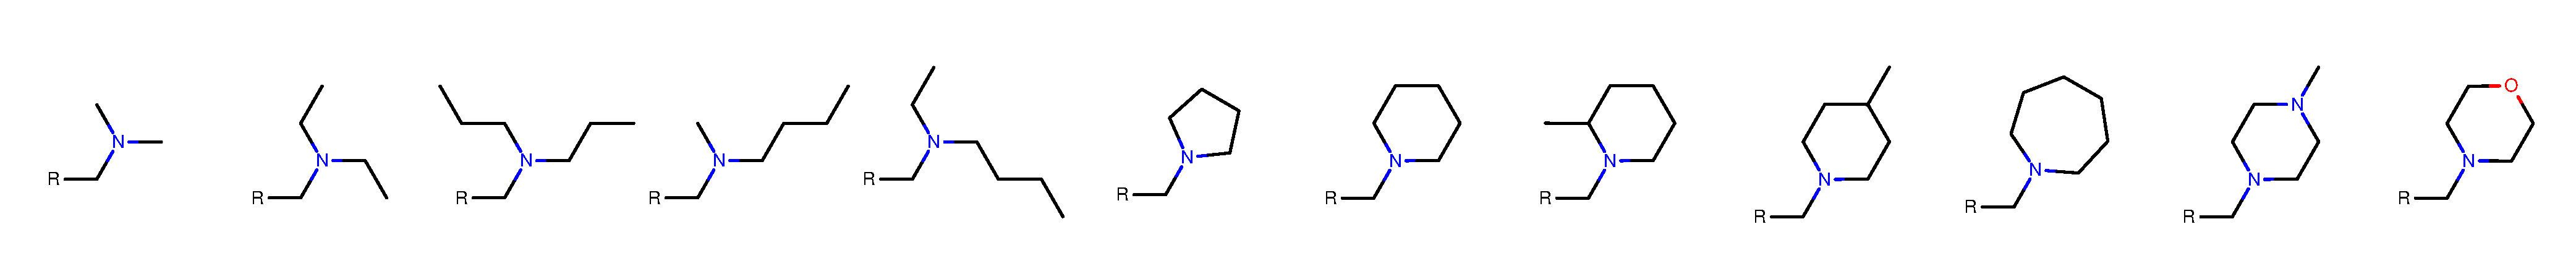
\includegraphics[width=\textwidth]{intercalators.pdf}
	\caption{A congeneric series of DNA intercalators. All molecules share a common quinoxaline scaffold. ~The experimental study was conducted by \cite{} producing binding affinity values that we could compare our calculations to. (Mention it in the experimental section)~ }
	\label{fig:intercalators}
\end{figure}


\section{Docking and scoring}

For certain application, like that of high throughput screening in the pharmaceutical industry, it is important to assess the binding strenght of a large number of drugs or molecules bound to large biological macromolecules like proteins or DNA in a very fast manner. This is done via easily evalutable scoring function, some notable examples including: AutoDock, X-Score, DrugScore, ChemScore, GOLD, FlexX, LigScore and LUDI. Generally speaking, they take into account a single structure and little or no protein movement is taking into account during evaluation. One of the simplest scoring function  consists of the empirical surface-area based method that shows that ligand binding reduces the surface are in the receptor that is accessible to the surrounding solvent. The function makes the assumption that the polar and non-polar area on the surface of the molecule has a linear relation to the free energy. Due to the crude simplifications in these models, they have weak predictive power and are rarely used for accurate free energy estimation. Here, a scoring methods is used for two reasons: (i) to find an initial structure for the intercalator-DNA complex, and (ii) to compare the scores and hence the ranking of this methods with other, more accurate models. Docking and scoring has its place in the drug discovery pipeline. In high throughput scenarios, where speed is an important factor due to the large number of molecules that need to be tested, scoring functions are often used to filter out candidates that have low probability of being good binders.

\subsection{Starting structures for docking}



\subsection{MMPBSA}

Molecular Mechanics Poisson-Boltzmann Surface Area (MMPBSA) is one of the theoretically approximate methods to calculate the free energy of system \cite{gilson2007calculation, steinbrecher2010towards}. It is the most accurate of the approximate methods, and it has previously been applied successfully to the free energy calculation of various biological systems including protein-ligand and DNA intercalator complexes.

This method is a good choice for comparing and ranking a set of molecule by their binding affinities for two main reasons: MMPBSA is able to handle a wide variety of systems and can the results can be theoretically calculated from a a single trajectory, unlike theoretically exact alchemical methods like FEP or TI. 

MMPBSA has become the a popular method to calculate binding affinities because of a balance between the details included in the physical model and the speed of the calculations themselves \cite{kollman2000calculating, sitkoff1994accurate}. As one of the main methods used in this thesis to calculate DNA-intercalator interactions, it will be discussed in more detail.

Applying the MMPBSA method to a system involves calculating the absolute free energy of binding by calculating three separate components: the free energies of the DNA-intercalator complex, the DNA and the intercalator molecules alone. The change is free energy upon intercalation then is

\begin{equation}
  \Delta G = \langle G_{complex} \rangle - \langle G_{DNA} \rangle - \langle G_{intercalator} \rangle
\end{equation}
\label{eq:mmpbsa}

where $\langle \dots \rangle$ represent the average value of a post-processing calculation performed on every frame of the simulation trajectory. Simulations are performed in explicit solvent and with counter-ions to balance the charge in the periodic simulation box.
To aid faster convergence of the free energy values the MMPBSA methods employs two strategies: first, all solvent molecules and counter-ions are replaced from the trajectory post simulation but pre-analysis by a continuum solvent approximation, and a thermodynamic cycle is used.

\subsubsection{The thermodynamic cycle}

\begin{figure}
  \centering
  \begin{tikzpicture}
  [ 
  waterbox/.style={rectangle,draw=blue!50,fill=blue!10,thick, inner sep=0pt,minimum size=5*\r},
  dna/.style={ultra thick, line cap=round},
  intercalator/.style={dna, dna, line width=3pt, blue},
  pre/.style={<-,shorten <=1pt,shorten >=1pt,semithick}, 
  post/.style={->,shorten <=1pt,shorten >=1pt,semithick}
  ]
  
  \node[waterbox] (a)               {};
  \node[waterbox] (b)  [right=of a] {}
    edge [pre] node[auto, swap] {$\Delta G_\text{b}^{aq}$} (a);
  \node[waterbox, fill=white] (a') [below=of a] {}
    edge [post] node[auto] {$\Delta G_\text{intercalator}^{sol}$} (a);
  \node[waterbox, fill=white] (b') [below=of b] {}
    edge [pre] node[auto] {$\Delta G_\text{b}^{vac}$} (a')
    edge [post] node[auto] {$\Delta G_\text{complex}^{sol}$} (b);
  \node[waterbox] (c)  [left=of a] {};
  \node[waterbox, fill=white] (c') [left=of a'] {}
    edge [post] node[auto] {$\Delta G_\text{dna}^{sol}$} (c);
    
  \node at ($(c.center)!0.5!(a.center)$) {+};
  \node at ($(c'.center)!0.5!(a'.center)$) {+};
  
  % \node[text width=10cm, align=center] [above=of a] {Thermodynamic cycle used to indirectly calculate the absolute free energy of intercalation};
  
  
  \foreach \x in {b.center, b'.center, c.center, c'.center} {
    \draw[dna]
      (\x) [rounded corners=\r] -- ++(-\s, 0) -- ++(0, 2*\s) 
      (\x) [rounded corners=\r] -- ++( \s, 0) -- ++(0, 2*\s)
      (\x) [rounded corners=\r] -- ++(-\s, 0) -- ++(0,-2*\s)
      (\x) [rounded corners=\r] -- ++( \s, 0) -- ++(0,-2*\s)
      
      (\x) ++(-0.866*\s,  0.5*\s) -- ++(1.73205*\s, 0)
      (\x) ++(   -\s,      \s) -- ++(   2*\s, 0)
      (\x) ++(   -\s,  1.5*\s) -- ++(   2*\s, 0)
      
      (\x) ++(-0.866*\s,  -0.5*\s) -- ++(1.73205*\s, 0)
      (\x) ++(      -\s,      -\s) -- ++(      2*\s, 0)
      (\x) ++(      -\s,  -1.5*\s) -- ++(      2*\s, 0);
  }
  
  \draw[intercalator] (a.center)  ++(-0.8*\s, 1.25*\s) -- ++(1.6*\s, 0);
  \draw[intercalator] (b.center)  ++(-0.8*\s, 1.25*\s) -- ++(1.6*\s, 0);
  \draw[intercalator] (a'.center) ++(-0.8*\s, 1.25*\s) -- ++(1.6*\s, 0);
  \draw[intercalator] (b'.center) ++(-0.8*\s, 1.25*\s) -- ++(1.6*\s, 0);

\end{tikzpicture}
  \caption{A solvation thermodynamic cycle is used to indirectly calculate the absolute binding free energy, $\Delta G_{b}^{aq}$, of an intercalator to the DNA in solvent. The rest of the free energy changes are calculated or estimated to then compute free energy of intercalation.}
  \label{fig:mmpbsacycle}
\end{figure}


\subsubsection{Single and Component trajectories}

The different contributions in equation \ref{eq:mmpbsa} can be extracted from a single trajectory of the complex, or from separate trajectories of the DNA, intercalator and complex. If a single trajectory is used, then the during the calculation of the different component, the rest of the system is removed and the analysis is done on part of the trajectory. This approach is effective in most scenarios and saves the additional cost of running multiple simulations for the separate components\cite{foloppe2006towards, wang2001use}. The other advantage of the single trajectory approach is that part of the complex that do not affect the intercalation cancel out exactly, as the coordinates are taken from the same trajectory, hence they are exactly the same. If separate trajectories are run for each component, than this error cancellation does not occur, as the component are free to explore different conformations. On the other hand, a single trajectory will not be able to capture dynamical changes to either the intercalator or, more importantly to the DNA, upon intercalation, and will consequently ignore certain contributions to the binding free energy. In the rest of the thesis, the three possible trajectory approaches are termed 1, 2 and 3 trajectory, corresponding to MMPBSA calculations where all three components are from the same simulation (1 trajectory), the intercalator is from a separate simulation (2 trajectory), or all three components, including the DNA are from three separate simulations (3 trajectory). 


\section{TIES}

The complexes of target DNA and hybrid intercalators were solvated in an orthorhombic water box with buffer width of 11 angstrom. The system was neutralized electrostatically with counterions. The BSC1\cite{ivani2016parmbsc1} force field was employed in all our simulations for DNA parameters. Intercalator parameters were produced using the general AMBER force field 2 (GAFF2) \cite{wang2004development}. The AM1BCC \cite{jakalian2002fast} %
semi-empirical methods was used to produce the partial charges on the intercalator atoms (AmberTools 18 \cite{ambertools18}) after geometry optimization with the OpenEye OEGauss toolkit. The simulation engine NAMD 2.12 was used for producing all the trajectories of the complex systems with periodic boundary conditions. The system was brought to and maintained at a temperature of 300 K and 1 atmosphere using the NAMD implementation of the Langevin thermostat (with a damping coefficient of $5 ps^{-1}$) and a Berendsen barostat (compressibility of $4.57 \times 10^{-5} bar^{-1}$ and a relaxation time of $100 fs$). The time step was set to $2 fs$. The van der walls terms perturbed linearly with respect to $\lambda$. To avoid end point catastrophes were atoms near the end point appear suddenly too close to each other a soft core potential was used for the van der Walls interactions. The electrostatic interactions of the disappearing atoms are linearly decoupled until $\lambda = 0.55$ then completely turned off afterwards, and those atoms that are appearing are electrostatically turned on from $\lambda = 0.45$ linearly increasing until the end.

All calculations were done with 13 $\lambda$ windows. At each value of $\lambda$ 5 replica simulations were run to assess the error. For each replica, the standard protocol for minimisation and equilibration was performed, that is 4 ns of simulation time. Production runs for each replica were 16 ns long. While the coordinates were recorded every 10 ps, $\partial V / \partial \lambda$ values were recorded every 2 ps. The choice of 16 ns for the simulation length and 5 for the ensemble size is based on the uncertainty quantification and error analysis discussed in the previous work. The protocol described here can be adjusted to the specific system at hand, but this was enough to converge results for all of the systems in this study. The size of the ensemble can be adjusted even at specific windows to account for additionally uncertainty that may arise. The TIES workflow can be executed in an embarrassingly parallel fashion, and given sufficient resources the simulations can finish in 15 hours. In general the turnaround time depends on the system size, number of cores used per simulation instance with GPUs offering additional speedup.



\chapter{Results and discussion}

This chapter describes and discusses the results. The results for each of the computational approaches to estimate either the binding free energy directly or range the intercalators is presented first, followed by a discussion of their relative merits.


\section{Docking and scoring}

The rigid planar scaffold of the intercalators that bind between DNA basepairs reduces the possible number of conformations that the docked structure can have. We have shown that using an extensive search method for docking, intercalators can be docked with RMSD less than $1$ angstrom for a wide range of intercalators compared to crystal structures.

We collected nine crystal structures of DNA-intercalator complex where the intercalator is between two consecutive basepairs. Table~\ref{tab:docking} shows the RMSD of every intercalator docked compared to the crystal structure. For seven of the cases docking is very close to the crystal structure, with average RMSD of $0.76$ angstrom. There are two cases where the docked structure is far from the reference.

After further investigating the outlier, the docked intercalators are in the correct place between the two basepairs, but their orientation is different from the one in the reference crystal structure. If there is no symmetry present in the intercalator molecule, then there are four possible orientations once docked. The free energy difference between these orientations is probably low, and the experimentally observed, dominant orientation is dependent of the kinetics of the intercalation too.

\begin{table}
  \caption{Results of docking nine intercalators compared to crystal structures We look at the root mean squared deviation of the heavy atoms from the reference positions in the PDB database.}
  \label{tab:docking}
  \centering
  \begin{tabular}{lS[round-mode=figures,round-precision=2]}
  \toprule
  {PDB ID} & {RMSD [angstrom]} \\
  \midrule
  1Z3F &  5.527405 \\
  1Z3F &  0.833399 \\
  1G3X &  0.593967 \\
  1HX4 &  1.195613 \\
  2ROU &  3.920575 \\
  1D11 &  0.586476 \\
  1D11 &  0.871855 \\
  1D12 &  0.401521 \\
  1D12 &  0.856238 \\
  \bottomrule
  \end{tabular}
\end{table}


The quinoxaline scaffold based intercalators were also docked and scored into the basepair opening of the 1Z3F crystal structure removing the original intercalated molecules.  

\begin{figure}
  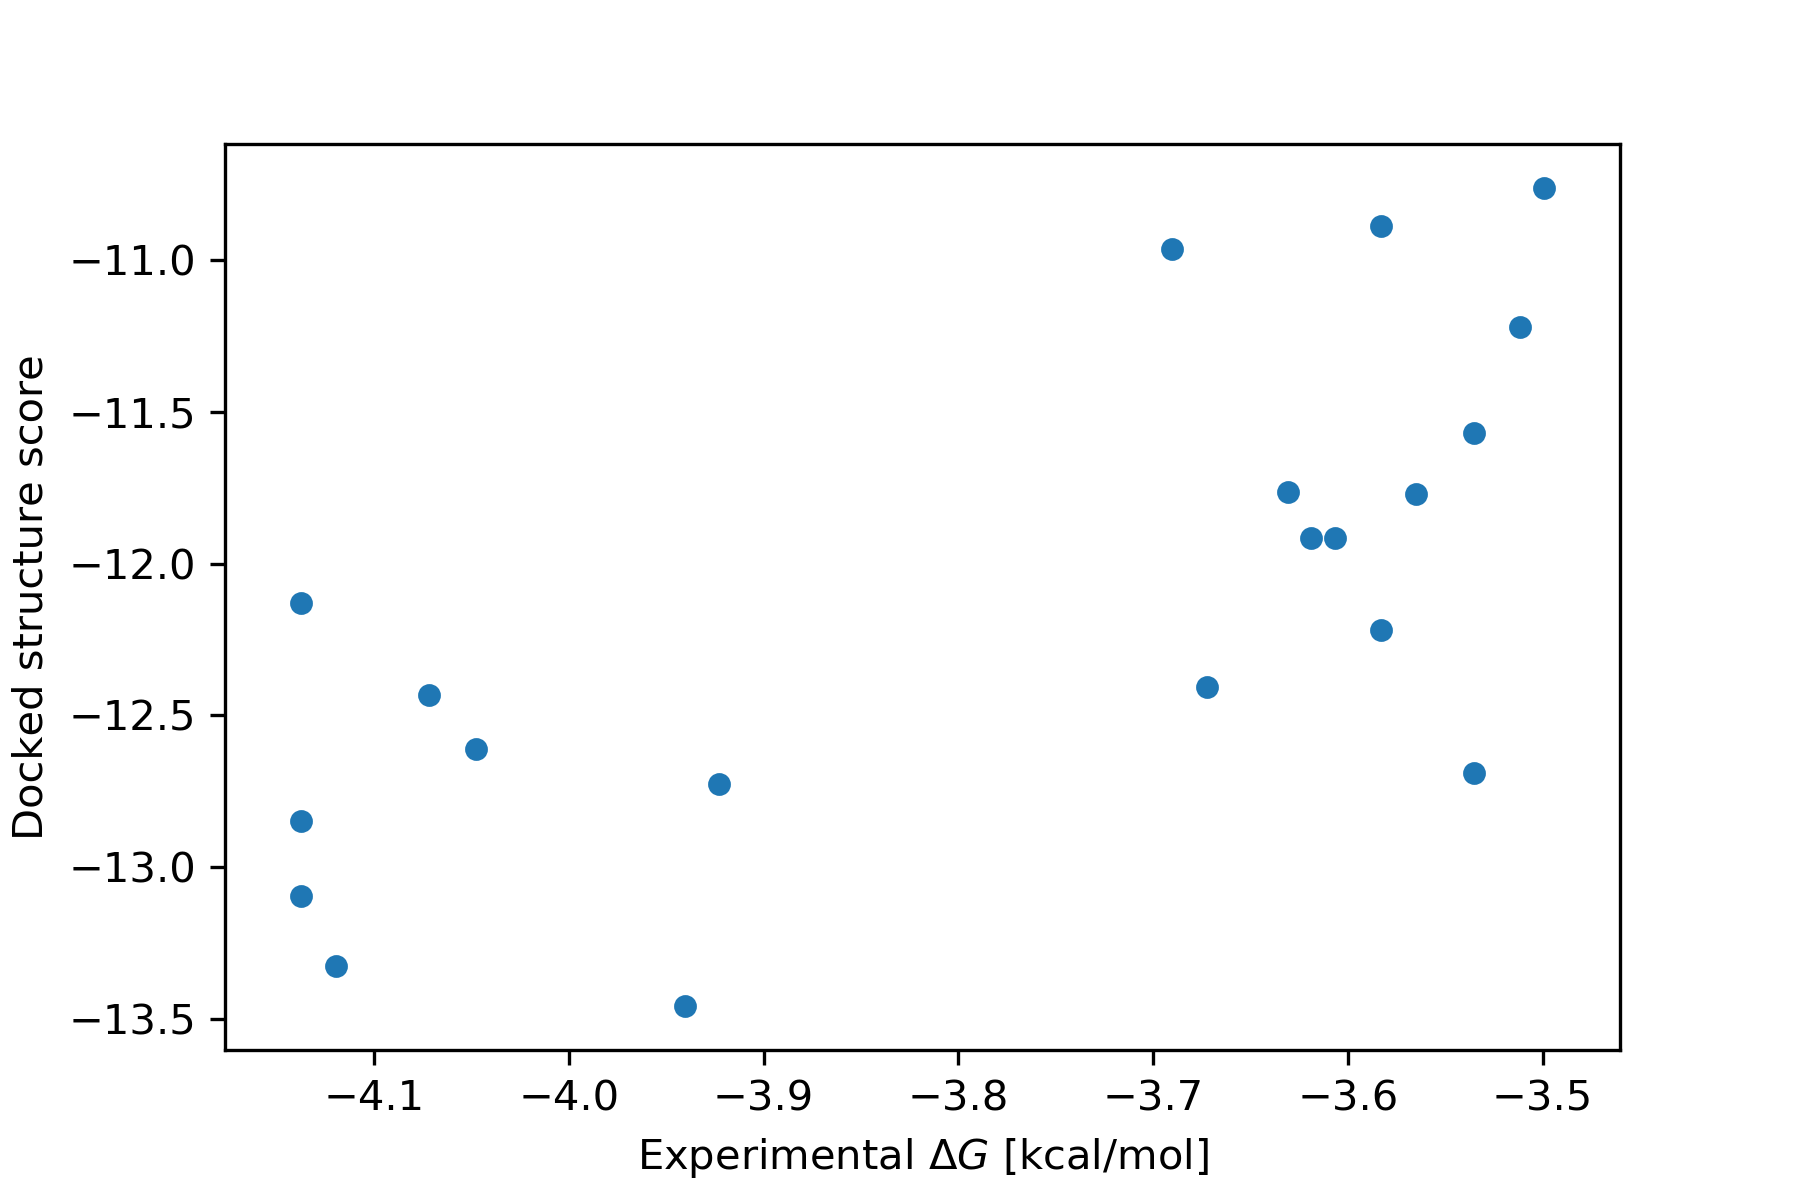
\includegraphics[width=\columnwidth]{docking}
  \caption{Plot of scores from docking the intercalators to the 1Z3F crystal structure. The ranking inside the 4 and 5 ring scaffold is poor, but there is a clear separation between the two intercalator types. This is in line with what we expect from the scoring method.}
  \label{fig:docking}
\end{figure}

\section{ESMACS}

In the past, there has been a number of MMPBSA type calculations for DNA intercalator systems. A large majority of these studies only takes into account just a few (one to three) intercalators binding to the DNA, and does not compare to experimental studies. We obtained a correlation Pearson coefficient of $r_p=0.70$ across the 10 planar molecules for the 3 trajectory calculation.

\subsubsection{Convergence}

It is important to assess the sampling efficiency and converge of the predicted free energy values in order for the results to be reliable and reproducible.
First, the comparison in convergence between a single trajectory approach and an ensemble of trajectories is compared for the MMPBSA and NMODE analysis methods in the context of free energy calculations. As the improvement in ensemble methods was evident, we investigated the length of each replica, extending the simulations from the original 5 ns simulation to 20 ns for each of the 25 replicas. It was important to sample the system long enough to cover a large part of the phase space, but not to oversample in places where the methods is no longer valid, for example during a de-intercalation pathway.

\subsubsection{Replica size and bootstrapped error}



\begin{figure}
  \begin{tikzpicture}
\begin{axis}[
  xlabel=Number of replicas,
  ylabel={Error (kcal/mol)},
  ]
  
  \addplot table {bootstrap.csv};
  
\end{axis}
\end{tikzpicture}
  \caption{Bootstrapped error as a function of replica size. }
  \label{fig:bootstrap}
\end{figure}

\subsubsection{Predicting the ranking}

The experimental free energy values are between \SIlist{-3.69;-3.50}{\kilo\calorie\per\mole}, making them hard to differentiate computationally. Approximate methods, like ESMACS, that are based on MMPBSA and NMODE for the free energy and entropy contribution, respectively do not have the resolution to differentiate experimental values at this scale. Nonetheless, correct error control and ensemble based calculations can give meaningful results relative to each other, i.e. ranking the intercalators based on their free energies will be comparable to experimental ranking.

% In methods talk about 1, 2, 3 trajectory

We have run 1, 2 and 3 trajectory calculations and as seen in Figure~\ref{fig:mmpbsa} the correlation improves, with the 3 trajectory being the most accurate with a correlation coefficient of $r_p=0.70$. The small interval of the experimental values suggests that the intercalators are very closely binding to the DNA. 

% This is a new subsection describing the energy components. P
% Check the 

The correlation achieved with ESMACS in this study suggests that one of the underlying forces (electrostatic, vdW, or internal energy) dominates the interaction gradient between the intercalators, and that signal is picked up by the MMPBSA calculation. Figure~\ref{fig:corrmat} shows the spread of the free energy values of the different components. Previous studies \cite{} have shown that vdW interactions contribute most to the binding energy of the intercalators in absolute terms. However, the correlation of the different components to the total binding energy shows that the internal energy (the sum of bond, angle, and torsion terms) correlate ~surprisingly~ with the total. 
% Induce fit, what it is?
This further supports our claim that the intercalation is an induced fit inside the two base-pairs.

% Methods
Each ESMACS calculation was run 25 times, the only difference being the random seed at the start of the simulation. 

% Beginning, quality of simulations, 
Variations in the results from the different replica was used to evaluate the error on the predicted free energy. Figure~\ref{fig:bootstrap} shows the bootstrapped error as a function of the number of replicas. There is a leveling off at around 20 replicas, with 25 replicas showing consistently low error bars.

% Energy contribution section
NMODE analysis was performed to include an approximation to the entropy contribution. Results show that including NMODE does not improve the ranking. 

% Convergence

% The original ESMACS protocol by \cite{} et al. 

\begin{figure}[h!]
	\documentclass[margin=0.1in]{article}

\usepackage{pgfplots}
\usepackage{pgfplotstable}
\pgfplotsset{compat=newest}


\usepackage{amsmath}
\usepackage{tikz}
\usetikzlibrary{positioning, calc}

\pgfmathsetmacro{\s}{0.5}
\pgfmathsetmacro{\r}{0.5cm}

\usepackage[caption=false]{subfig}

\begin{document}

\begin{figure}
  
\subfloat{%
\begin{tikzpicture}%3traj
\begin{axis}[
  scale=0.7,
  xtick distance = {0.1},
  ytick distance = {1},
  %xlabel={\phantom{nothing}}, 
  %ylabel={Calculated $\Delta$G (\si{\kilo\calorie\per\mole})},
  legend pos=south east]
  
  \addplot[blue!70!white] table [col sep=comma, x=exp, y={create col/linear regression={y=dg_3_traj}}] {4-ring-mmpbsa.csv};
  % \addplot[red!70!white] table [col sep=comma, x=exp, y={create col/linear regression={y=dg_3_traj_nmode}}] {4-ring-mmpbsa.csv};

  \addplot[blue, mark=*, only marks, error bars/.cd,
          x dir=both, x explicit,
          y dir=both, y explicit,] table 
          [col sep=comma, x=exp, y=dg_3_traj, y error=dg_3_traj_err, x error=exp_err] {4-ring-mmpbsa.csv};
  % \addplot[red, mark=*, only marks, error bars/.cd,
  %         x dir=both, x explicit,
  %         y dir=both, y explicit,] table[col sep=comma, x=exp, y=dg_3_traj_nmode, y error=dg_3_traj_err, x error=exp_err] {4-ring-mmpbsa.csv};
  
  \legend{3 trajectory, $R=0.70$}%, w/ n-mode}

\end{axis}  
\end{tikzpicture}%
}
\subfloat{%
\begin{tikzpicture}%3traj-nmode
\begin{axis}[
  scale=0.7,
  xtick distance = {0.1},
  ytick distance = {1},
  %xlabel={\phantom{nothing}}, 
  %ylabel={Calculated $\Delta$G (\si{\kilo\calorie\per\mole})},
  legend pos=south east]
  
  \addplot[red!70!white] table [col sep=comma, x=exp, y={create col/linear regression={y=dg_3_traj_nmode}}] {4-ring-mmpbsa-failednmode.csv};
  % \addplot[red!70!white] table [col sep=comma, x=exp, y={create col/linear regression={y=dg_3_traj_nmode}}] {4-ring-mmpbsa.csv};

  \addplot[red, mark=*, only marks, error bars/.cd,
          x dir=both, x explicit,
          y dir=both, y explicit,] table 
          [col sep=comma, x=exp, y=dg_3_traj_nmode, y error=dg_3_traj_err, x error=exp_err] {4-ring-mmpbsa-failednmode.csv};
  % \addplot[red, mark=*, only marks, error bars/.cd,
  %         x dir=both, x explicit,
  %         y dir=both, y explicit,] table[col sep=comma, x=exp, y=dg_3_traj_nmode, y error=dg_3_traj_err, x error=exp_err] {4-ring-mmpbsa.csv};
  
  \legend{3 trajectory + nmode, $R=0.62$}%, w/ n-mode}

\end{axis}  
\end{tikzpicture}
}

\subfloat{%
\begin{tikzpicture}%2traj
\begin{axis}[
  scale=0.7,
  xtick distance = {0.1},
  ytick distance = {1},
  %xlabel=Experimental $\Delta$G (\si{\kilo\calorie\per\mole}), 
  %ylabel={Calculated $\Delta$G (\si{\kilo\calorie\per\mole})},
  legend pos=south east
  ]
  
  \addplot[blue!70!white] table [col sep=comma, x=exp, y={create col/linear regression={y=dg_2_traj}}] {4-ring-mmpbsa.csv};    
  % \addplot[red!70!white] table [col sep=comma, x=exp, y={create col/linear regression={y=dg_2_traj_nmode}}] {4-ring-mmpbsa.csv};

  \addplot[blue, mark=*, only marks, only marks, error bars/.cd,
          x dir=both, x explicit,
          y dir=both, y explicit,] table[col sep=comma, x=exp, y=dg_2_traj, y error=dg_2_traj_err, x error=exp_err] {4-ring-mmpbsa.csv};
  % \addplot[red, mark=*, only marks, only marks, error bars/.cd,
  %         x dir=both, x explicit,
  %         y dir=both, y explicit,] table[col sep=comma, x=exp, y=dg_2_traj_nmode, y error=dg_2_traj_err, x error=exp_err] {4-ring-mmpbsa.csv};
  \legend{2 trajectory, $R=0.64$}%, w/ n-mode}

\end{axis}  
\end{tikzpicture}%
}
\subfloat{%
\begin{tikzpicture}%2traj-nmode
\begin{axis}[
  scale=0.7,
  xtick distance = {0.1},
  ytick distance = {1},
  %xlabel=Experimental $\Delta$G (\si{\kilo\calorie\per\mole}), 
  %ylabel={Calculated $\Delta$G (\si{\kilo\calorie\per\mole})},
  legend pos=south east
  ]
  
  \addplot[red!70!white] table [col sep=comma, x=exp, y={create col/linear regression={y=dg_2_traj_nmode}}] {4-ring-mmpbsa-failednmode.csv};    
  % \addplot[red!70!white] table [col sep=comma, x=exp, y={create col/linear regression={y=dg_2_traj_nmode}}] {4-ring-mmpbsa.csv};

  \addplot[red, mark=*, only marks, only marks, error bars/.cd,
          x dir=both, x explicit,
          y dir=both, y explicit,] table[col sep=comma, x=exp, y=dg_2_traj_nmode, y error=dg_2_traj_err, x error=exp_err] {4-ring-mmpbsa-failednmode.csv};
  % \addplot[red, mark=*, only marks, only marks, error bars/.cd,
  %         x dir=both, x explicit,
  %         y dir=both, y explicit,] table[col sep=comma, x=exp, y=dg_2_traj_nmode, y error=dg_2_traj_err, x error=exp_err] {4-ring-mmpbsa.csv};
  \legend{2 trajectory + nmode, $R=0.50$}%, w/ n-mode}

\end{axis}  
\end{tikzpicture}
}

\subfloat{%
\begin{tikzpicture}%1traj
\begin{axis}[
  scale=0.7,
  xtick distance = {0.1},
  ytick distance = {1},
  %xlabel={\phantom{nothing}}, 
  %ylabel={Calculated $\Delta$G (\si{\kilo\calorie\per\mole})},
  legend pos=south east
  ]
  
  \addplot[blue!70!white] table [col sep=comma, x=exp, y={create col/linear regression={y=dg_1_traj}}] {4-ring-mmpbsa.csv};    
  % \addplot[red!70!white] table [col sep=comma, x=exp, y={create col/linear regression={y=dg_2_traj_nmode}}] {4-ring-mmpbsa.csv};

  \addplot[blue, mark=*, only marks, only marks, error bars/.cd,
          x dir=both, x explicit,
          y dir=both, y explicit,] table[col sep=comma, x=exp, y=dg_1_traj, y error=dg_1_traj_err, x error=exp_err] {4-ring-mmpbsa.csv};
  % \addplot[red, mark=*, only marks, only marks, error bars/.cd,
  %         x dir=both, x explicit,
  %         y dir=both, y explicit,] table[col sep=comma, x=exp, y=dg_2_traj_nmode, y error=dg_2_traj_err, x error=exp_err] {4-ring-mmpbsa.csv};
  \legend{1 trajectory, $R=0.64$}%, w/ n-mode}
\end{axis}  
\end{tikzpicture}%
}
\subfloat{%
\begin{tikzpicture}%1traj-nmode
\begin{axis}[
  scale=0.7,
  xtick distance = {0.1},
  ytick distance = {1},
  %xlabel={\phantom{nothing}}, 
  %ylabel={Calculated $\Delta$G (\si{\kilo\calorie\per\mole})},
  legend pos=south east
  ]
  
  \addplot[red!70!white] table [col sep=comma, x=exp, y={create col/linear regression={y=dg_1_traj_nmode}}] {4-ring-mmpbsa-failednmode.csv};    
  % \addplot[red!70!white] table [col sep=comma, x=exp, y={create col/linear regression={y=dg_2_traj_nmode}}] {4-ring-mmpbsa.csv};

  \addplot[red, mark=*, only marks, only marks, error bars/.cd,
          x dir=both, x explicit,
          y dir=both, y explicit,] table[col sep=comma, x=exp, y=dg_1_traj_nmode, y error=dg_1_traj_err, x error=exp_err] {4-ring-mmpbsa-failednmode.csv};
  % \addplot[red, mark=*, only marks, only marks, error bars/.cd,
  %         x dir=both, x explicit,
  %         y dir=both, y explicit,] table[col sep=comma, x=exp, y=dg_2_traj_nmode, y error=dg_2_traj_err, x error=exp_err] {4-ring-mmpbsa.csv};
  \legend{1 trajectory + nmode, $R=0.39$}%, w/ n-mode}
\end{axis}  
\end{tikzpicture}
}
\end{figure}

\end{document}
	\caption{Correlation between one (bottom), two (middle) and three (top) trajectory calculations and experiment. Values are presented for NMODE (red) analysis and without NMODE (blue). The best Pearson correlation is for the NMODE-less values starting from \num{0.64} for the 1, and 2 trajectory and \num{0.70} for the 3 trajectory. The NMODE calculations have a Pearson correlation of \numlist{0.39; 0.5; 0.62} for the 1, 2, and 3 trajectory calculations respectively.}
	\label{fig:mmpbsa}
\end{figure}


\section{TIES}

Relative alchemical free energy calculations were done between five pairs of the intercalator from the original experimental study. As discussed above, there are two groups of intercalator there: the four and five membered ring scaffolds. Pairs were selected based on two criteria: first to maximise the experimental free energy difference and second to sample all three possible combinations of transformation (between the 4 ring systems, 5 ring systems, and a transformation from 4 ring to 5 ring). 

As seen in figure~\ref{fig:ties} the correlation to experiment is poor. This can be for a number of reasons, but investigating more systems could be insightful. The experimental results for this study indicate binding affinities that are very close to each other, and even the best methods will struggle to differentiate between them. In the future we will collect and simulate intercalator ligand systems with experimental free energy differences large enough to be probed computationally. The simulations do converge as seen in figure~\ref{fig:ties_conv} well before the end of the simulation time. Still, TIES does produce more accurate results then the more approximate methods like ESMACS or docking. The root mean squared error on this small set of transformations is 0.41 kcal/mol.

\begin{figure}
  \centering
  \begin{tikzpicture}
\begin{axis}[
  ylabel=Predicted $\Delta \Delta G$,
  xlabel=Experimental $\Delta \Delta G$,
  ]
  
  \addplot[blue, mark=*, only marks] table {ties.csv};
  
\end{axis}  
\end{tikzpicture}
  \caption{Correlation plot comparing the experiment free energy difference with the calculated values via TIES. The experimental values are too close to each other, and the difference is smaller than the resolution of the TIES method given the 5 replicas used here. Furthermore the experimental error becomes large when we take the free energy difference between two values.}
  \label{fig:ties}
\end{figure}

\begin{figure}
  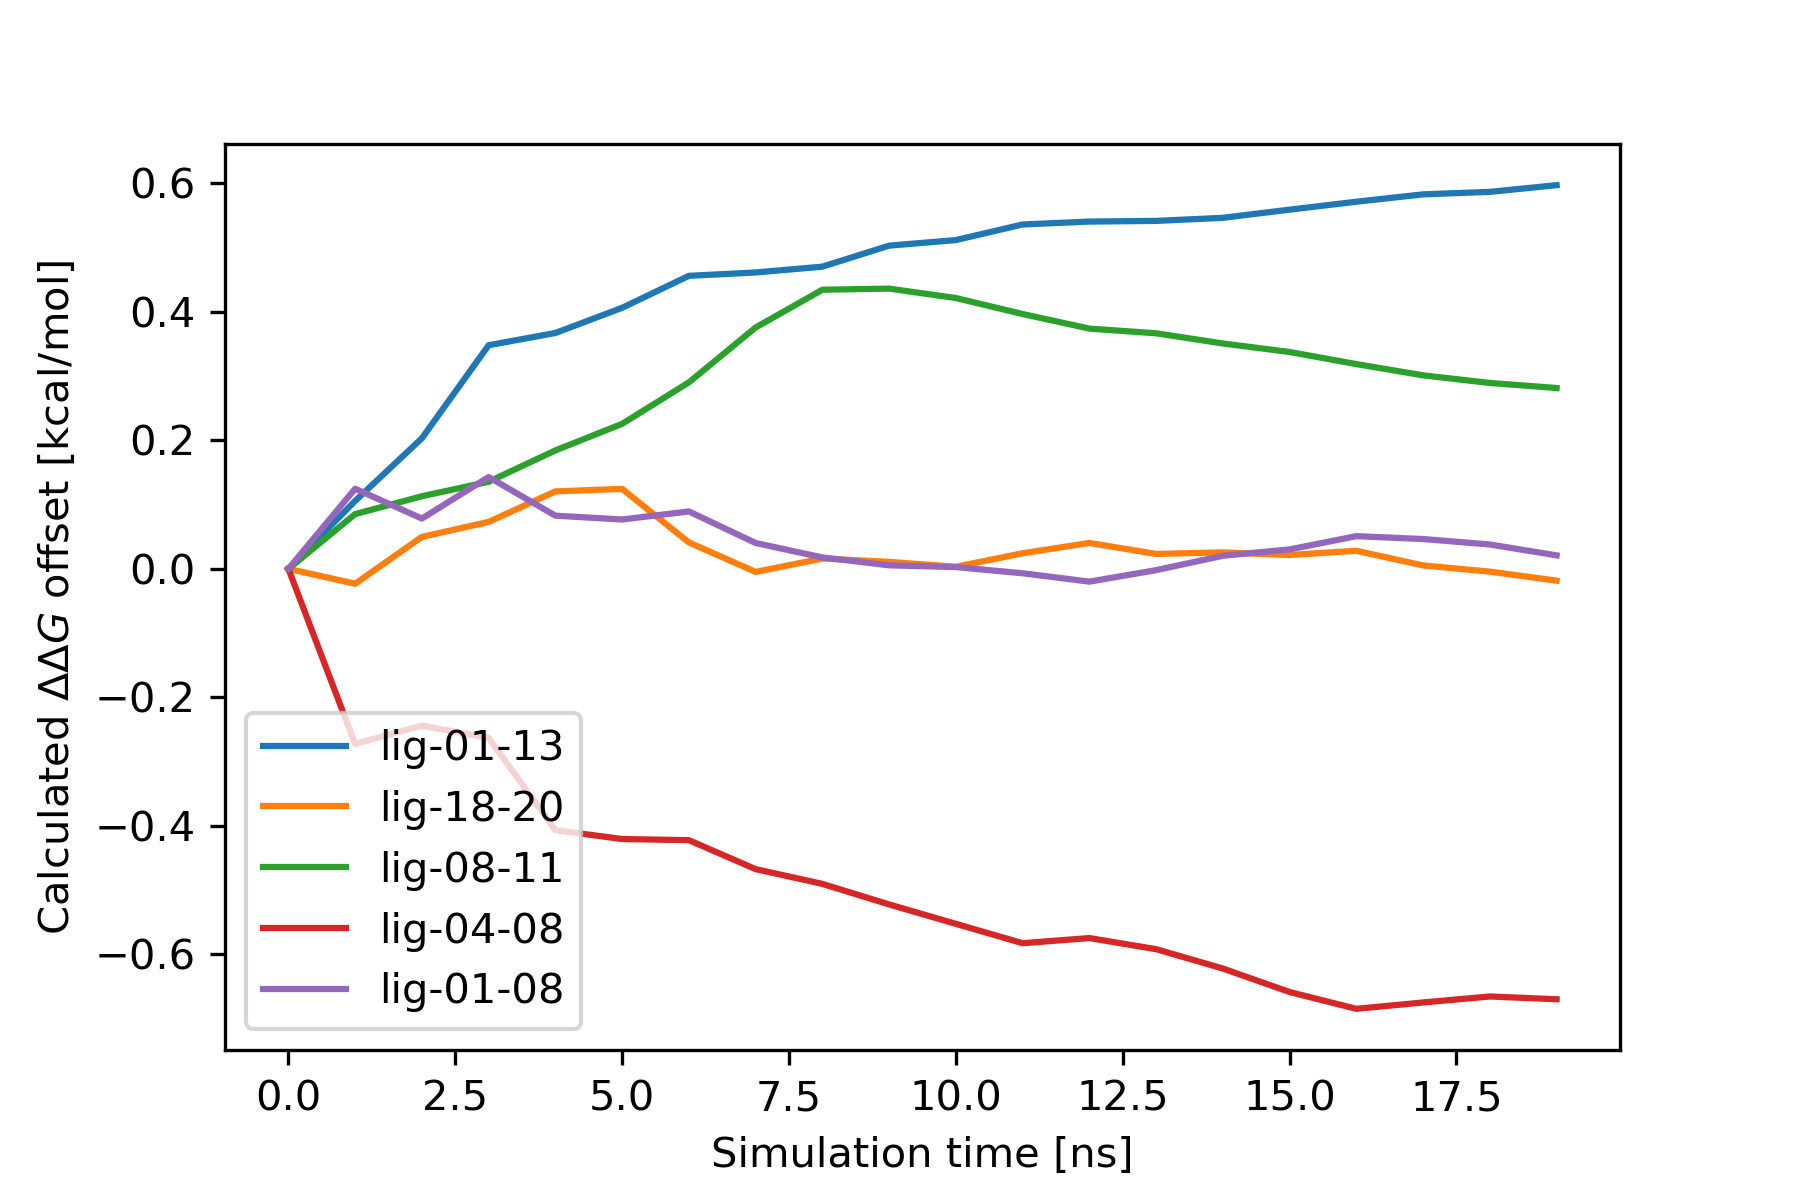
\includegraphics[width=\columnwidth]{ties_conv.png}
  \caption{Time evolution of the free energy difference for the five intercalator pairs investigated. The results are levelled off indicating that we reached converged values. The values are offset so they all start at point zero for illustrative purposes.}
  \label{fig:ties_conv}
\end{figure}



\chapter{Conclusion}


%\bibliography{mybib}
%\bibliographystyle{plain}

\end{document}